%%%%%%%%%%%%%%%%%%%%%%%%%%%%%%%%%%%%%%%%%%%%%%%%%%%%%%%%%%%%%%%%%%%%%%%%%%%%%%%%
%2345678901234567890123456789012345678901234567890123456789012345678901234567890
%        1         2         3         4         5         6         7         8

\documentclass[10pt, conference]{IEEEtran}

%\overrideIEEEmargins                                      % Needed to meet printer requirements.

%In case you encounter the following error:
%Error 1010 The PDF file may be corrupt (unable to open PDF file) OR
%Error 1000 An error occurred while parsing a contents stream. Unable to analyze the PDF file.
%This is a known problem with pdfLaTeX conversion filter. The file cannot be opened with acrobat reader
%Please use one of the alternatives below to circumvent this error by uncommenting one or the other
%\pdfobjcompresslevel=0
%\pdfminorversion=4

% See the \addtolength command later in the file to balance the column lengths
% on the last page of the document

% The following packages can be found on http:\\www.ctan.org
\usepackage{graphicx}
%\usepackage{graphics} % for pdf, bitmapped graphics files
%\usepackage{epsfig} % for postscript graphics files
%\usepackage{mathptmx} % assumes new font selection scheme installed
%\usepackage{times} % assumes new font selection scheme installed
\usepackage{amsmath} % assumes amsmath package installed
\usepackage{amssymb}  % assumes amsmath package installed
\usepackage{bm} % for bold symbols in math mode
\usepackage{cite}

\title{\LARGE \bf
Report: SLIP models for controlling articulated robotic legs
}


\author{Stefan Schneyer and Fabian Kolb}

\begin{document}
\maketitle
\thispagestyle{empty}
\pagestyle{empty}


%%%%%%%%%%%%%%%%%%%%%%%%%%%%%%%%%%%%%%%%%%%%%%%%%%%%%%%%%%%%%%%%%%%%%%%%%%%%%%%%
%\begin{abstract} TODOabstract \end{abstract}

\section{Introduction}


Bio inspired robotics and especially humanoid robots play an increasing role in society and science. Robotic solutions with a structural 
similarity to humans are especially suitable for tasks which are up to now mainly solved by humans. For moving in challenging terrain with higher velocities
hopping is an interesting approach. For simplicity hopping can be simulated with one leg. SLIP models describe the spring-like leg behaviour
of animals and humans in a very simple and abstract way. The model reduces the leg to a massless spring with a point mass attached to the top. 
This abstract SLIP model behaviour is then projected on the dynamics of an articulated leg. 
In a first stage a closed loop dynamics is generated based on the SLIP model. In the second stage the high order robotic leg tracks this closed loop dynamics 
and uses a feedback controller to adapt to deviations. The robot state is modelled as automaton. A continuous state captures the position of the 
robot in the 3D space, the hip angle and knee angle. A discrete state models the transition of flight to stance and stance to flight phase. 
A control structure is implemented for both the flight and the stance phase. 
For the flight phase a cascade control consisting of PI and PID controller is used. When touching the ground, the SLIP dynamics can be 
projected onto the CoG motion of the robotic leg. From there the joint actuator torques which are necessary to generate the operational space 
forces is calculated. Real robotic legs differ from the simplified SLIP model because the mass and inertia of the leg's segments influence the 
the robot's motion. Real robots suffer from the impact when the foot strikes the ground. This leads to a loss of kinetic energy which is incorperated in 
the SLIP model by an energy compensation. Different types of integration are implemented in order to study their effect on the controller stability. 
The project is implemented in Python. The RBDL library is used, which offers efficient rigid body dynamics algorithms. 
For visualization Meshup, a tool that was developed with RBDL is used.




\section{SLIP model}
The SLIP model is an abstraction capturing the locomotion behavior of robots with light, compliant legs. In this model the body is reduced to a point mass \( m \). The
leg is represented by a massless spring with stiffness \({k}_0 \) and a rest length \({l}_0 \). For this system the equations of motion are the following:
\begin{equation}
   \begin{bmatrix} m & 0 \\ 0 & m \end{bmatrix}
   \begin{bmatrix} \ddot{x} \\ \ddot{y} \end{bmatrix}
   +
   \begin{bmatrix} 0 \\ mg \end{bmatrix}
   =
   \begin{bmatrix} {F}_{x} \\ {F}_{y} \end{bmatrix}
\end{equation}

where x and y are the coordinates of the center of mass (COM). \({F}_x \) and \({F}_y \) are the ground reaction forces (GRF). The GRFs are 0 during flight and depend 
on the length of the spring \(l\) during compression and the landing angle \(\alpha\) of the foot.

\begin{equation}
   \begin{bmatrix} {F}_{x}  \\ {F}_{y}  \end{bmatrix}
   =
   {k}_{0} ({l}_{0} -l)
   \begin{bmatrix} -cos(\alpha) \\ sin(\alpha) \end{bmatrix}
\end{equation}

The SLIP model describes running as a series of apex heights \({y}_i \)

\begin{figure}[h]
   \centering
   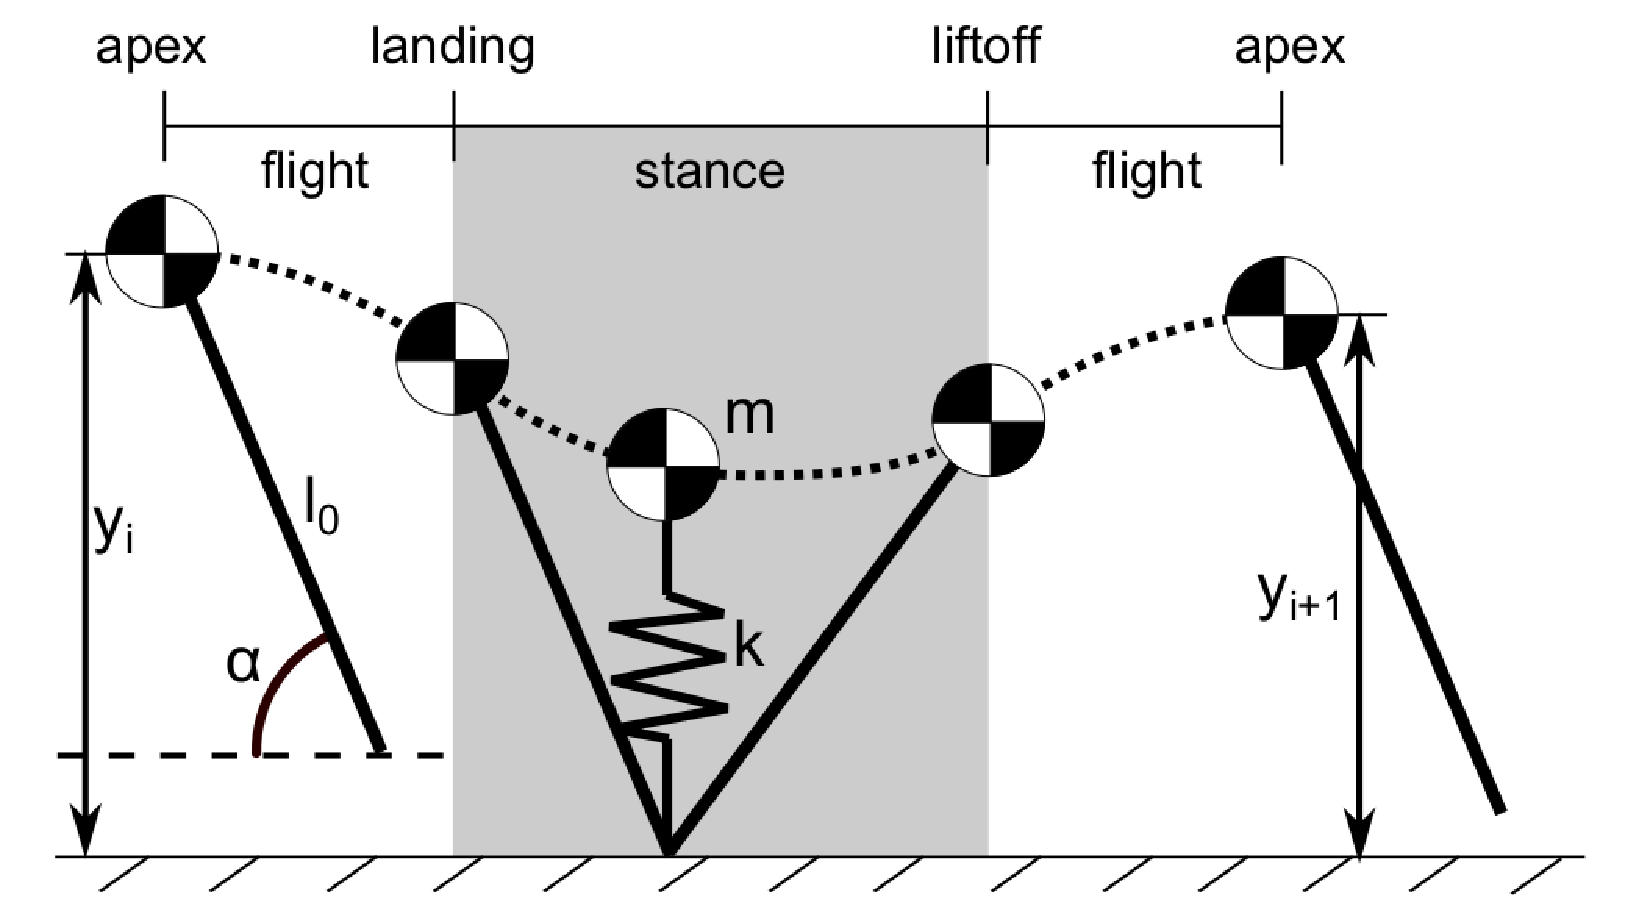
\includegraphics[scale=0.2]{"assets/SMM2.pdf"}
   \caption{flight and stance phases of SLIP model \cite{Wu2014}}
   \label{fig_SLIP_phase}
\end{figure}


In Fig. \ref{fig_SLIP_phase} it becomes clear how the robot trajectory can be separated in flight and stance phases. The gait behavior is characterized by the forward speed and the apex height.
The SLIP model is a conservative system without any friction or other mechanism to dissipate the dynamics, and thus, their phase space does not shrink over time. 
Therefore, the apex height and forwards speed are coupled through the system energy and the trajectory is fully characterized by the apex height. 
The transition between two consecutive apex heights is defined by the landing angle \(\alpha\):
\begin{equation}
   {f}_{yi+1}={f}_{yi}|(\alpha)
\end{equation}
The landing angle is used to achieve deadbeat stability of the system \cite{Wu2014} \cite{Hutter2010}.




\section{Control}








\subsection{Higher order model: ATRIAS}

The ATRIAS robot has lightweight carbon fiber legs. The robots total mass is concentrated mostly in the trunk. The legs are constructed as a four bar structure actuated 
by two motors through a leaf spring. The leaf springs and the four bar structure of each leg generate spring like forces in the legs. These spring like forces and 
the fact that the trunk outweigh the legs make the SMM abstraction especially useful for the ATRIAS robot.

\begin{figure}[h]
   \centering
   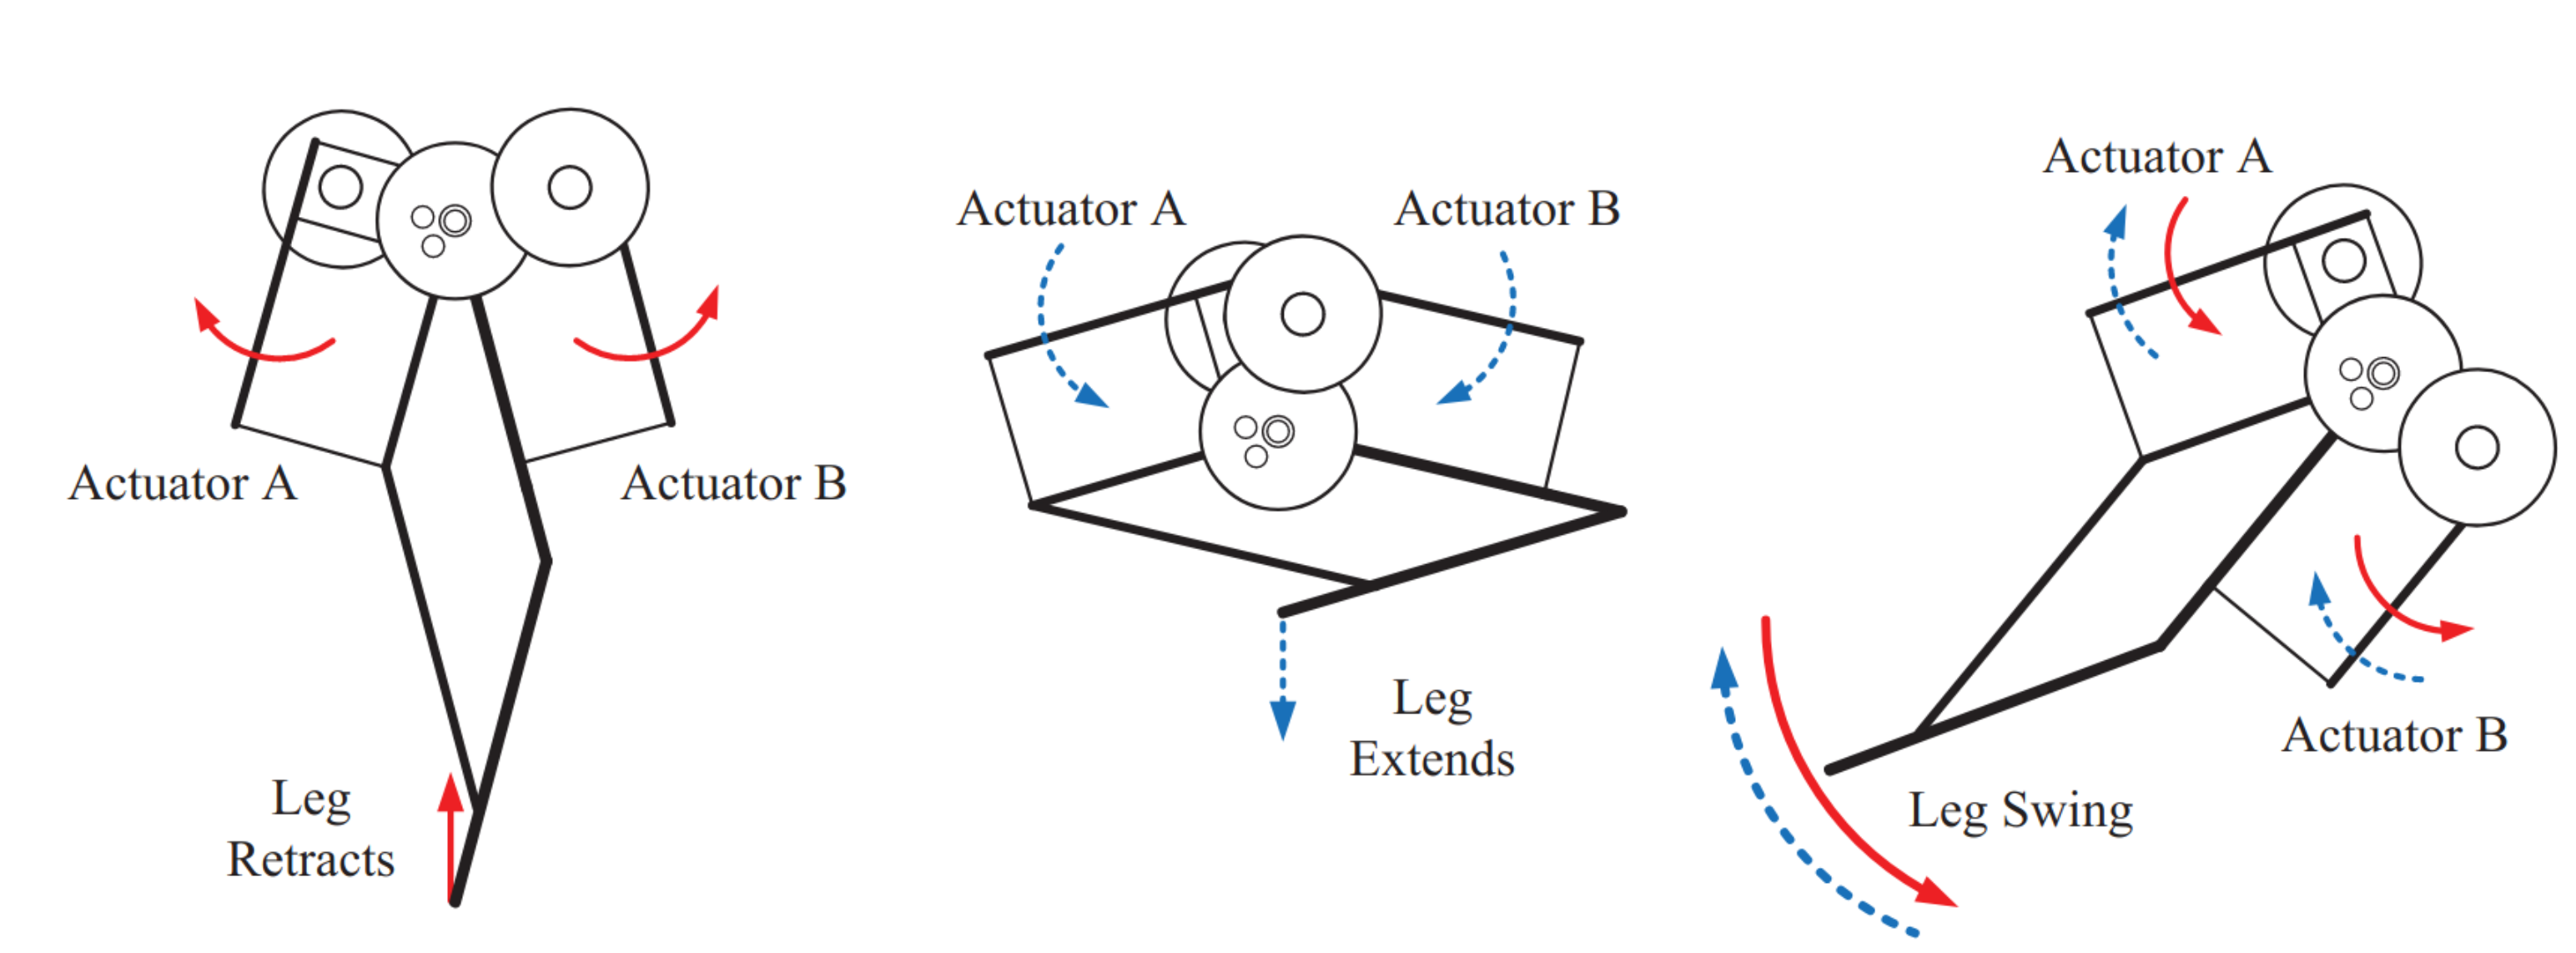
\includegraphics[scale=0.07]{"assets/ATRIAS2.png"}
   \caption{ATRIAS leg actuation \cite{Grimes2012}}
   \label{fig_ATRIAS_motion}
\end{figure}


The pair of motors allow changing the orientation and length of the leg (Fig. \ref{fig_ATRIAS_motion}). The motors can generate linear actuator outputting forces \({F}_{i} \) and rotatory torques
 \({\tau}_{i} \).  

\begin{figure}[h]
   \centering
   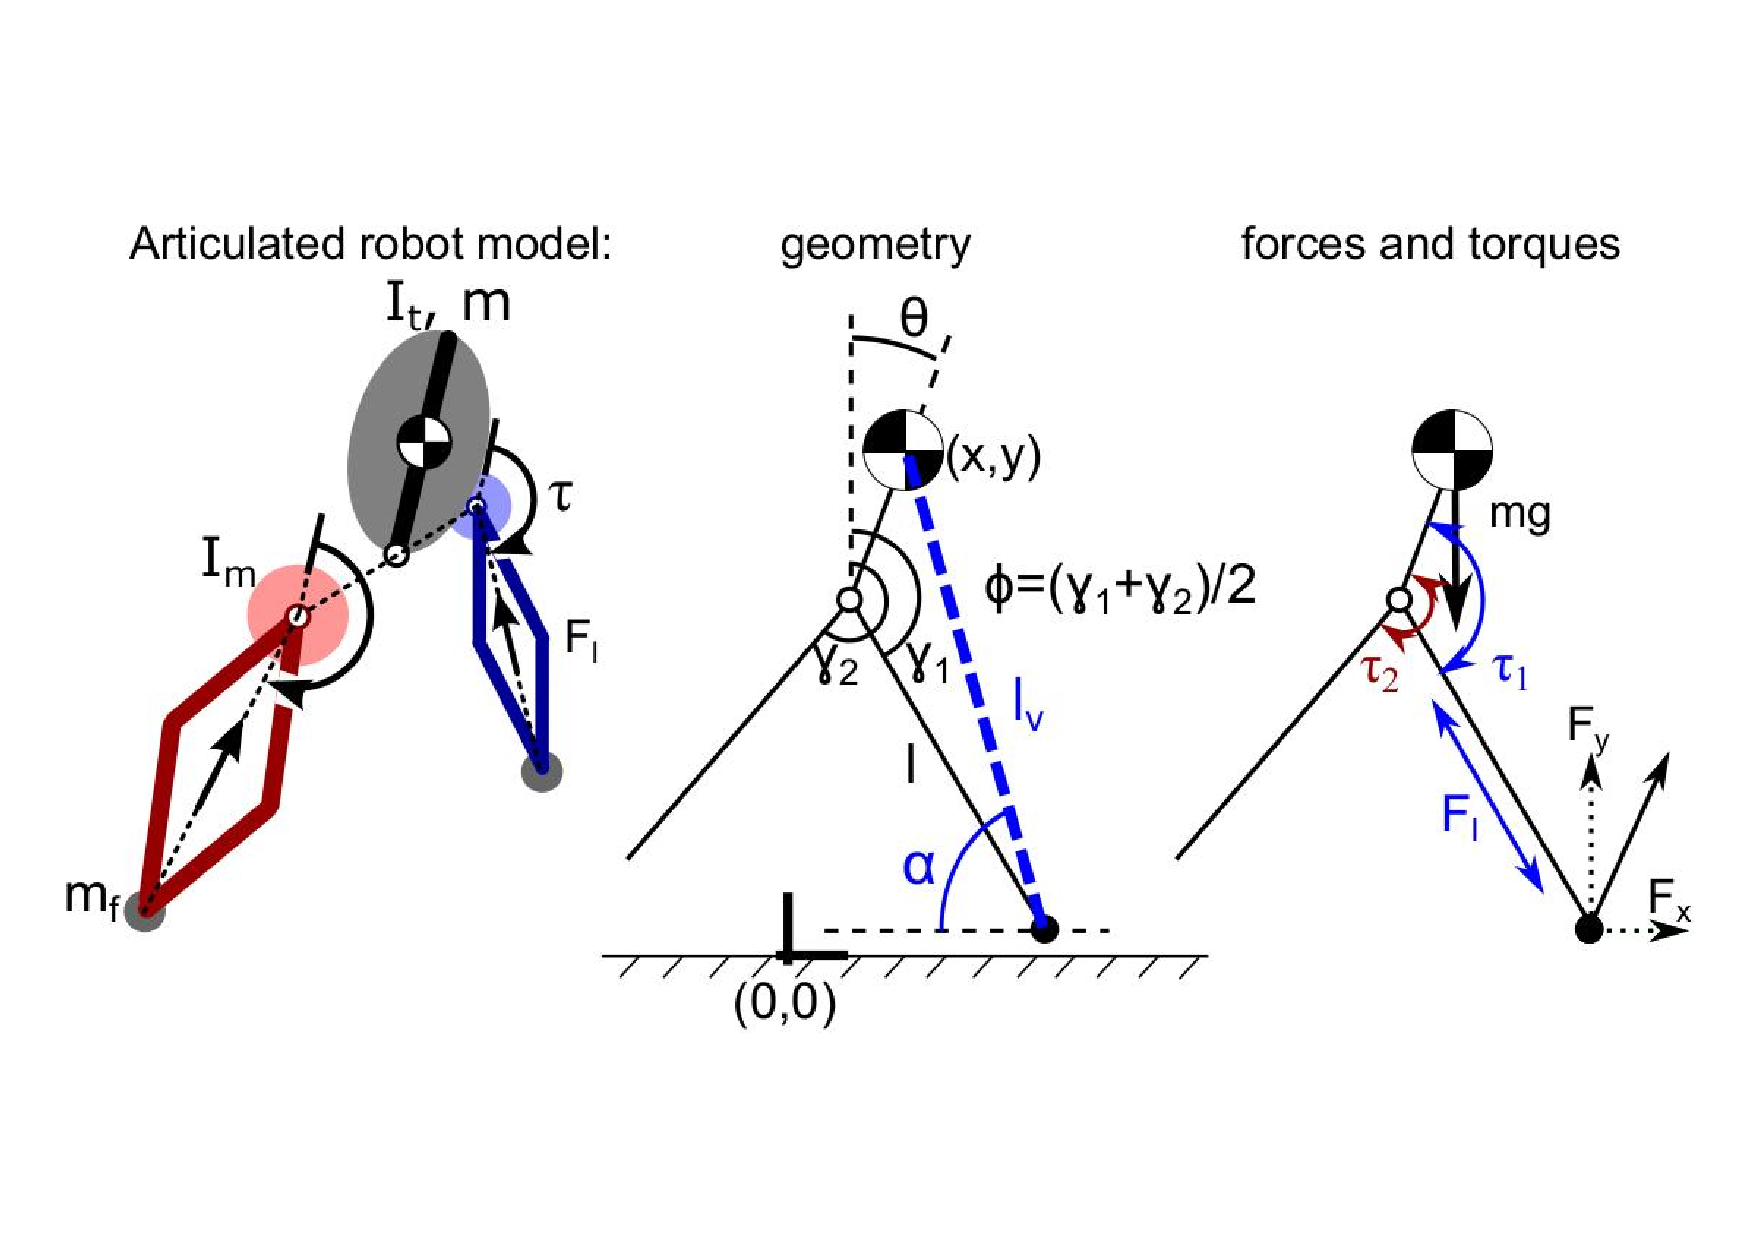
\includegraphics[scale=0.23]{"assets/ATRIAS1.pdf"}
   \caption{ATRIAS model \cite{Wu2014}}
   \label{fig_ATRIAS}
\end{figure}

In contrast to the SMM abstraction, the ATRIAS robot also needs to balance the trunk, generate swing motion in order to move the legs during flight phase and 
consider slip at the feed dissipating the system energy. The model of the ATRIAS robot is shown in Fig. \ref{fig_ATRIAS}. In vertical direction a GRF is generated
corresponding to a spring damper system. In horizontal direction a sliding force proportional to the vertical GRF is generated opposing the motion of 
the robot. The dynamics of the ATRIAS robot can be described by the equation of motion:
\begin{equation}
   M(q)\ddot{q}+h(q,\dot{x}))=S{\tau}+{J}^TF 
\end{equation}
where M is the mass matrix, q is the coordinate vector, h accounts for Coriolis, centrifugal and gravitational forces, the selection matrix S assigns control inputs 
\({\tau}\) to \(q\). The coordinate vector consists of the global position and orientation of the trunk \(x\), \(y\), \({\theta}\) and the global orientation and 
length of each leg \({\gamma}_i\), \({l}_i\). The control vector \({\tau}\) consists of motor torques \({\tau}_i\) and linear force \({F}_i\) of each leg \cite{Wu2014} \cite{Grimes2012}.       

\section{Mapping and control design}
For controlling the ATRIAS robot a few assumptions were applied. Since the mass of the feet is clearly smaller than the mass of the robot, the inertial effects of 
the feet can be neglected. This assumption does eliminate the dynamics of the leg during flight. The force for swinging the leg during flight is controlled separately 
and is not part of the paper. Besides that it is assumed that there is no slip during the whole stance phase \cite{Wu2014}.

\subsection{Control Goals}
Based on the SMM model the leg placement policy \({\alpha}(t)\) provides deadbeat tracking of the robot gait, which is fully determined by the apex height. The ATRIAS 
robot is able to achieve the same performance when tracking the landing angle and generating GRFs through the center of mass (COM) corresponding to the spring forces 
in the SMM. To prevent unstable trunk pitch rates, the angular momentum  \(H={I}_{t}\dot{\theta}+{I}_m\dot{\gamma}_{1}{I}_m\dot{\gamma}_{2}\) around the COM should be 
stabilized at zero in average. This is achieved by keeping the trunk pitch constant 
at \({\theta}^{*}\) and mirroring the hip angle velocities \(\dot{\gamma}_{1} = -\dot{\gamma}_{2}\). Also, the translational Energy 
\({E}_{Trans}=\frac{1}{2}m(\dot{x}^{2}+\dot{y}^{2})+mgy\) should match the system energy \({E}^{*}\) that parametrizes the SMM. Since the inertial effects 
of the feet are ignored \(H\) and \({E}_{Trans}\) can only be regulated during stance. Besides that the robot feet should not be trailed back too far \({\gamma}_{2}=2{\pi}-{\gamma}_{1}\). 
The average hip angle is therefore \(\frac{{\gamma}_{1}+{\gamma}_{2}}{2}={\pi}\) \cite{Wu2014}.
\subsection{Flight}
During flight the COM follows on the calculated trajectory and no external forces are applied on the robot. The control focuses on the angular motions of the 
trunk, hips and legs and minimizes their error to \({\theta}^{*}\), \({\phi}^{*}\), \({\alpha}^{*}\). An LQR controller is used to find an optimal trade off between these goals \cite{Wu2014}.
\subsection{Stance}
During the stance phase the trunk pitch \({\theta}\),  average hip angle \({\phi}\) and translational energy \({E}_{Trans}\) are tracked. The GRFs are calculated from the SMM and also tracked. To achieve the control goals, a cascade control design is used \cite{Wu2014}. 
\subsubsection{Outer loop}
Target GRFs are aimed such that they produce work reducing the system energy error between \({E}_{Trans}\) and \({E}^{*}\). Since spring-leg behavior is assumed 
virtual spring forces are calculated to model the robot's GRFs \cite{Wu2014}.
\subsubsection{Inner loop}
Actuator commands are calculated from these virtual spring forces to produce the actual robot GRFs defined in the outer loop. To do so, the virtual spring forces are 
substituted in the equations of motion to solve for the feed-forward actuation \([{\tau}_{1,ff}, {\tau}_{2,ff}, {F}_{1,ff}]\). These produce the work opposing the estimated 
energy error from the outer loop. In a feedback loop torques are calculated driving the average hip angle \({\phi}\) and trunk pitch \({\theta}\) towards their stationary references \({\pi}\) and \({\theta}^{*}\).
\begin{equation}
   \label{eq:t}
   \begin{aligned}
   {\tau}_{2,fb}={K}_{p{\phi}}(2{\pi}{\gamma}_{1}-{\gamma}_{2})-{K}_{d{\phi}}(\dot{{\gamma}_{1}}+\dot{{\gamma}_{2}})\\
   {\tau}_{1,fb}=-{\tau}_{2,fb}+{K}_{p0}({\theta}_{*}-{\theta}){K}_{d0}(\dot{\theta})
   \end{aligned}
\end{equation}
For the motor torques the feed-forward and feedback results are added \({\tau}_{i}={\tau}_{i,ff}+{\tau}_{i,fb}\) and for the leg force just the feedforward actuation is used \({F}_{i}={F}_{i,ff}\) \cite{Wu2014}.

\section{Results}
\begin{figure}[h]
   \centering
   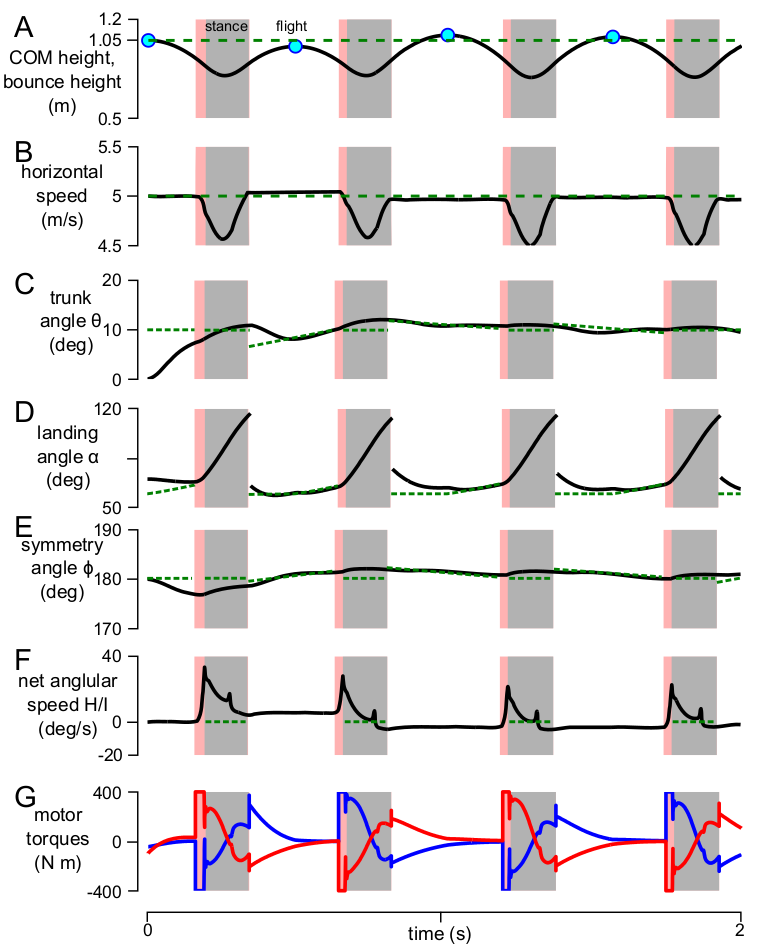
\includegraphics[scale=0.34]{"assets/results.pdf"}
   \caption{First two seconds of running in flat terrain \cite{Wu2014}}
   \label{results}
\end{figure}

Fig. \ref{results} shows the performance of the control design for the ATRIAS robot on flat ground. C and E show that the controller is able to stabilize the trunk pitch 
\({\theta}\) and the average hip angle \({\phi}\) in two steps. These can still deviate from their goal angle in order to stabilize the angular momentum H. 
The gait behavior described by the apex height in A and forward velocity in B was achieved by matching the landing condition \({\alpha}^{*}(t)\). 
When the foot slips (red shaded in G) maximum torque is applied in order to oppose the motion of the foot. When the foot is stationary (gray shaded in G) the applied torques generate GRFs in order to regulate the
 system energy and to drive the angular momentum H towards zero \cite{Wu2014}.

\addtolength{\textheight}{-12cm}   % This command serves to balance the column lengths
                                  % on the last page of the document manually. It shortens
                                  % the textheight of the last page by a suitable amount.
                                  % This command does not take effect until the next page
                                  % so it should come on the page before the last. Make
                                  % sure that you do not shorten the textheight too much.

\nocite{*}
\bibliographystyle{IEEEtran}
\bibliography{IEEEabrv, report}

\end{document}
